\documentclass[9pt,a4paper,twoside]{../rho-class/rho}
\usepackage{ctex}
\usepackage{amsmath}
\usepackage{amssymb}
\usepackage{siunitx}
\usepackage{hyperref}
\usepackage{indentfirst}
\usepackage{fontspec}

\setmainfont{Noto Serif CJK SC}
\setsansfont{Noto Sans CJK SC}

\setbool{rho-abstract}{true} % Set false to hide the abstract
\setbool{corres-info}{false} % Set false to hide the corresponding author section
\setbool{linenumbers}{false} % Set false to hide the line numbering

\sisetup{
    mode = math, 
    reset-math-version = false, 
}
\setlength{\parindent}{2em}
\linespread{1.2}

\addbibresource{rho.bib}

%----------------------------------------------------------
% TITLE
%----------------------------------------------------------

\journalname{大学物理-基础实验B 实验报告}
\title{单摆法测重力加速度 \  实验报告}

%----------------------------------------------------------
% AUTHORS AND AFFILIATIONS
%----------------------------------------------------------

% \author[1,$\dagger$]{崔俊熙}
% \author[2,$\ddagger$]{实验主管老师}
% \author[2,$\ddagger$]{实验助教}
\author{崔俊熙 PB25000124}

%----------------------------------------------------------

% \affil[1]{中国科学技术大学少年班学院}
% \affil[2]{中国科学技术大学物理学院}
% \affil[$\dagger$]{学号: PB25000124.}
% \affil[$\ddagger$]{实验指导教师.}

%----------------------------------------------------------
% DATES
%----------------------------------------------------------

% \dates{本篇实验报告收稿于2026年XX月XX日，于2026年XX月XX日提交.}
\dates{2026-03-24}

%----------------------------------------------------------
% FOOTER INFORMATION
%----------------------------------------------------------

\leadauthor{崔俊熙 PB25000124}
\footinfo{大学物理-基础实验B 实验报告}
\smalltitle{单摆法测重力加速度 \  实验报告}
\institution{中国科学技术大学}
\theday{2026-03-24} %\today

%----------------------------------------------------------
% ARTICLE INFORMATION
%----------------------------------------------------------

% \corres{Provide the corresponding author information and publisher here.}

\email{cuijunxi@mail.ustc.edu.cn.}

% \received{March 20, 2024}
% \revised{April 16, 2024}
% \accepted{April 20, 2024}
% \published{May 21, 2024}

% \license{Rho LaTeX Class \ccLogo\ This document is licensed under Creative Commons CC BY 4.0.}

\hypersetup{
    pdftitle={单摆法测重力加速度 实验报告},
    pdfauthor={崔俊熙},
    pdfsubject={大学物理-基础实验B 实验报告},
    pdfkeywords={单摆法; 重力加速度; 累积放大法; 不确定度分析},
    pdfcreator={LaTeX},
    pdfproducer={XeLaTeX}
}

%----------------------------------------------------------
% ABSTRACT
%----------------------------------------------------------

\begin{abstract}
    本实验旨在利用单摆法测量当地的重力加速度$g$.
    实验基于单摆在小摆角条件下的简谐运动原理, 通过测量有效摆长$l$ (摆线长与摆球半径之和)及$N$个周期的累积时间$t$, 结合一级近似周期公式进行计算.
    为了满足实验精度优于$\qty{1}{\percent}$的要求, 本研究通过不确定度分析确定了合理的测量方案,
    即采用累积放大法测量至少25个周期降低秒表启停时人为反应时间带来的不确定度.
    实验过程中分别对摆长和周期进行了6次重复测量,并利用标准不确定度合成公式对结果进行了评估.
\end{abstract}

%----------------------------------------------------------

\keywords{ 关键词 单摆法; 重力加速度; 累积放大法; 不确定度分析}

%----------------------------------------------------------

\begin{document}

\maketitle
\thispagestyle{firststyle}
% \tableofcontents

%----------------------------------------------------------

\section{引言}
\rhostart{单}摆实验是一个经典实验, 许多著名的物理学家如伽利略, 牛顿, 惠更斯等都对单摆实验进行过细致的研究.
伽利略发现了摆的等时性原理, 指出摆的周期与摆长的平方根成正比, 而与摆的质量和材料无关, 为后来摆钟的设计与制造奠定了基础.
1673年荷兰科学家惠更斯制造的惠更斯摆钟就运用了摆的等时性原理.
摆的等时性原理应用于时钟上, 作为稳定的``定时器'', 使机械钟能够指示出``秒'', 从而将计时精度提高了近100倍.
现在国际上采用铯原子的跃迁周期作为计时标准, 由中国计量科学研究院研制的NIM6铯原子钟, 其不确定度优于$5.8 \times 10^{-16}$, 相当于5400万年不差一秒. \cite{jiangyi}



\section{实验仪器与实验原理}

\subsection{实验仪器}

钢卷尺; 电子秒表; 单摆(带标尺,平面镜；摆线长度可调,其可调的上限约为\qty{100}{\centi\metre}); 智能手机(自备). \cite{jiangyi}

\begin{figure}[H]
    \centering
    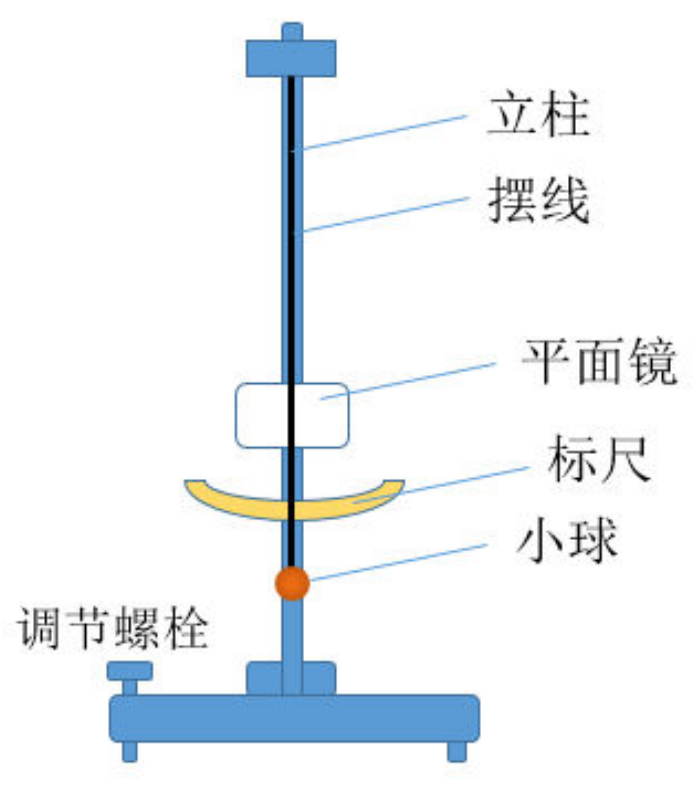
\includegraphics[width=0.72\columnwidth]{1.png}
    \caption{单摆实验装置}
\end{figure}

\subsection{实验原理}

理想的单摆, 是一根没有质量, 没有弹性的线, 系住一个没有体积的质点,
在真空中由于重力作用而在与地面垂直的平面内做摆角趋于零的自由振动. 这种理想的单摆, 实际上是不存在的.
在实际的单摆实验中, 悬线是一根有质量(弹性很小)的线, 摆球是有质量有体积的刚性小球, 摆角不为零, 摆球的运动还受到空气的影响. \cite{jiangyi}

\subsubsection{运动学原理}

在摆角$\theta < 5^\circ$, 忽略空气浮力及摆线质量的一级近似条件下, 单摆运动可视为简谐运动, 其周期公式为
\begin{equation}
    T = 2\pi\sqrt{\frac{l}{g}}
\end{equation}

其中, $l$为有效摆长(摆线长与摆球半径之和), $T$为摆动周期.
由此可导出重力加速度计算公式
\begin{equation}
    g = \frac{4\pi^2 l}{T^2}
\end{equation}

\subsubsection{不确定度分析推导}

对重力加速度公式进行偏导分析
\begin{equation}
    \frac{\partial g}{\partial l} = \frac{4\pi^2}{T^2} = \frac{g}{l}, \quad \frac{\partial g}{\partial T} = -\frac{8\pi^2 l}{T^3} = -\frac{2g}{T}
\end{equation}

根据误差传递公式, 合成不确定度$u_g$为
\begin{equation}
    u_g = \sqrt{\left( \frac{\partial g}{\partial l} u_l \right)^2 + \left( \frac{\partial g}{\partial T} u_T \right)^2} = g \sqrt{\left( \frac{u_l}{l} \right)^2 + \left( \frac{2u_T}{T} \right)^2}
\end{equation}

即相对不确定度传递公式为
\begin{equation}
    \frac{u_g}{g} = \sqrt{\left( \frac{u_l}{l} \right)^2 + \left( \frac{2u_T}{T} \right)^2}
\end{equation}

\begin{rhoenv}[frametitle=Attention.]
    \begin{itemize}
        \item 有效摆长的不确定度来自钢卷尺测量摆线的误差, 以及游标卡尺测量小球直径的误差.
              其中钢卷尺的误差为$\qty{0.2}{\centi\metre}$, 游标卡尺的误差为$\qty{0.02}{\centi\metre}$.
              因此$u_l \approx \sqrt{(\qty{0.2}{\centi\metre})^2 + (\qty{0.02}{\centi\metre})^2} \approx \qty{0.2}{\centi\metre}$.

        \item 周期的不确定度来自秒表的误差以及实验人员的反应时间.
              其中秒表的误差为$\qty{0.1}{\second}$, 实验人员的反应时间误差为$\qty{0.2}{\second}$.
              因此$u_T \approx \sqrt{(\qty{0.1}{\second})^2 + (\qty{0.2}{\second})^2} \approx \qty{0.22}{\second}$.
    \end{itemize}
\end{rhoenv}

\subsubsection{测量周期数}

为了使实验精度达到$\frac{u_g}{g} \leqslant \qty{1}{\percent}$, 我们需要确定重复测量周期数$N$.
当摆长$l = \qty{70}{\centi\metre}$时, 取$g = \qty{9.8}{\metre\per\second\squared}$, 得单次周期$T = \qty{1.68}{\second}$.
若仅测量单次周期, 相对不确定度约为$\qty{23.8}{\percent}$.

考虑重复测量$N$个周期, 此时不确定度变为
\begin{equation}
    \frac{u_g}{g} = \sqrt{\left( \frac{u_l}{l} \right)^2 + \left( \frac{2u_T}{NT} \right)^2} \approx \sqrt{\left( 0.00286 \right)^2 + \left( \frac{0.262}{N} \right)^2}
\end{equation}

令$\frac{u_g}{g} \leqslant \qty{1}{\percent}$, 解得$N \geqslant 25$, 即至少要测量25个周期.

\section{实验过程}
\subsection{实验内容}

\begin{enumerate}
    \item 固定摆长测量周期, 重复测量6次.
    \item 改变摆长测量周期, 测量6组不同的摆长和周期.
\end{enumerate}

\begin{rhoenv}[frametitle=Attention.]
    \begin{itemize}
        \item 待单摆稳定摆动后, 再开始计时.
        \item 摆动幅度不要过大, 控制摆角不大于$5^{\circ}$.
        \item 不要数错周期数.
    \end{itemize}
\end{rhoenv}

\section{实验结果与讨论}

\subsection{实验数据}

\begin{table}[H]
    \centering
    \begin{tabular}{|c|c|c|c|c|c|c|}
        \hline
        $L$ / \unit{\centi\metre} & 68.10                    & 68.10 & 68.10 & 68.10 & 68.09 & 68.17 \\ \hline
        $T$ / \unit{\second}      & 41.35                    & 41.18 & 41.40 & 41.42 & 41.46 & 41.33 \\ \hline
        $N$                       & \multicolumn{6}{|c|}{25}                                         \\ \hline
    \end{tabular}
    \caption{固定摆长, 重复测量周期}
    \label{tab:table-1}
\end{table}

\begin{table}[H]
    \centering
    \begin{tabular}{|c|c|c|c|c|c|c|}
        \hline
        $L$ / \unit{\centi\metre} & 68.10                    & 62.23                    & 72.80 & 44.50 & 50.02 & 37.38 \\ \hline
        $T$ / \unit{\second}      & 41.42                    & 39.53                    & 42.78 & 53.40 & 56.96 & 48.96 \\ \hline
        $N$                       & \multicolumn{3}{|c|}{25} & \multicolumn{3}{|c|}{40}                                 \\ \hline
    \end{tabular}
    \caption{更改摆长, 测量周期}
    \label{tab:table-2}
\end{table}

其中, $L$为有效摆长, $T$为测量时间, $N$为测量周期数.

\subsection{数据分析}

\subsubsection{重复测量数据处理}
根据Table \ref{tab:table-1} 的数据, 对6次重复测量的有效摆长$L$和25个周期的总时间$T$取平均值：
\begin{itemize}
    \item 平均有效摆长: $\overline{l} \approx \qty{68.11}{\centi\metre} = \qty{0.6811}{\metre}$
    \item 平均单次周期: $\overline{T} \approx \qty{1.654}{\second}$
\end{itemize}

计算重力加速度测量值：
\begin{equation}
    g = \frac{4\pi^2 \overline{l}}{\overline{T}^2} \approx \frac{4 \times \pi^2 \times 0.6811}{1.654^2} = \qty{9.8240}{\metre\per\second\squared}
\end{equation}

\subsubsection{变摆长回归分析(利用Table \ref{tab:table-2})}
根据$4 \pi^2 \cdot L = g \cdot \frac{T^2}{N^2}$, 以$\frac{T^2}{N^2}$为横轴, $4 \pi^2 \cdot L$为纵轴进行最小二乘线性回归, 斜率$k = g$.
通过表 \ref{tab:table-2} 中6组不同摆长的数据计算得 $\tilde{g} = \qty{9.7765}{\metre\per\second\squared}$.

\section{实验结论与思考}

\subsection{实验结论}

本实验通过单摆法测量了实验室环境下的重力加速度$g$. 实验采用了两种数据处理方法:
\begin{itemize}
    \item \textbf{平均值法(固定摆长)}: 通过对6次重复测量数据的平均处理, 计算得到重力加速度$g_1 = \qty{9.8240}{\metre\per\second\squared}$.
    \item \textbf{线性回归法(变摆长)}: 利用6组不同摆长的数据, 以 $T^2/N^2$ 为横轴, $4\pi^2 \cdot L$为纵轴进行最小二乘拟合, 得到斜率即重力加速度$g_2 = \qty{9.7765}{\metre\per\second\squared}$.
\end{itemize}

\subsection{思考题}

\paragraph{Question.} 分析实验测量误差的主要来源, 提出可能的改进方案.

\paragraph{Answer.} 本实验的误差主要来源于以下几个方面:
\begin{enumerate}
    \item \textbf{摆角影响}: 理论公式$T = 2\pi\sqrt{\frac{l}{g}}$是在$\theta \to 0$的一级近似下得出的.
          实际摆角(如$5^\circ$)会导致周期偏大, 从而使计算出的$g$值偏小.
    \item \textbf{摆线质量与空气浮力}: 实验忽略了摆线的质量以及空气对摆球的浮力.
          摆线质量会使摆动中心上移, 有效摆长变短; 空气浮力则会减小回复力, 等效于减小了$g$.
    \item \textbf{计时操作}: 尽管采用了累积放大法($N \geqslant 25$), 但秒表的启停仍存在约$\qty{0.2}{\second}$的人为反应延迟.
    \item \textbf{长度测量}: 钢卷尺测量摆线长时, 若尺面未完全垂直或未能精准对齐摆动支点, 会产生测量偏差.
\end{enumerate}

\paragraph{改进方案：}
\begin{itemize}
    \item \textbf{使用传感器计时}: 采用光电门传感器连接数字毫秒计, 可消除人为反应时间误差, 将计时精度提高到$\qty{0.001}{\second}$.
    \item \textbf{周期修正}: 引入更高阶的周期公式$T = 2\pi\sqrt{\frac{l}{g}}\left( 1 + \frac{1}{4}\sin^2\frac{\theta}{2} + \dots \right)$, 并测量起始摆角进行修正.
    \item \textbf{Tracker 软件分析}: 利用手机拍摄摆动视频, 使用 Tracker 视频分析插件记录摆动轨迹, 通过运动学拟合直接获取周期和摆角, 减少人工计数错误.
\end{itemize}

\section{致谢}

感谢中国科学技术大学物理实验教学中心提供的实验设备与讲义指导;
感谢实验老师和助教在数据记录规范与不确定度分析逻辑上给予的耐心指导;
感谢搭档在实验过程中的配合.

\printbibliography

\section*{附录：包含签字的实验原始数据}

\begin{figure}[H]
    \centering
    \includegraphics[width=0.72\columnwidth]{2.png}
    \caption{包含签字的原始数据}
\end{figure}

\end{document}